\documentclass{article}

\usepackage{fancyhdr}
\usepackage{extramarks}
\usepackage{amsmath}
\usepackage{amsthm}
\usepackage{amsfonts}
\usepackage{tikz}
\usepackage{url}
\usepackage[plain]{algorithm}
\usepackage{algpseudocode}
\usepackage{hyperref}
\usetikzlibrary{automata,positioning}

%
% Basic Document Settings
%

\topmargin=-0.45in
\evensidemargin=0in
\oddsidemargin=0in
\textwidth=6.5in
\textheight=9.0in
\headsep=0.25in

\linespread{1.1}

\pagestyle{fancy}
\lhead{\hmwkAuthorName}
\chead{\hmwkClass\ (\hmwkTitle}
\rhead{\firstxmark}
\lfoot{\lastxmark}
\cfoot{\thepage}

\renewcommand\headrulewidth{0.4pt}
\renewcommand\footrulewidth{0.4pt}

\setlength\parindent{0pt}

%
% Create Problem Sections
%

\newcommand{\enterProblemHeader}[1]{
    \nobreak\extramarks{}{Problem \arabic{#1} continued on next page\ldots}\nobreak{}
    \nobreak\extramarks{Problem \arabic{#1} (continued)}{Problem \arabic{#1} continued on next page\ldots}\nobreak{}
}

\newcommand{\exitProblemHeader}[1]{
    \nobreak\extramarks{Problem \arabic{#1} (continued)}{Problem \arabic{#1} continued on next page\ldots}\nobreak{}
    \stepcounter{#1}
    \nobreak\extramarks{Problem \arabic{#1}}{}\nobreak{}
}

\setcounter{secnumdepth}{0}
\newcounter{partCounter}
\newcounter{homeworkProblemCounter}
\setcounter{homeworkProblemCounter}{1}
\nobreak\extramarks{Problem \arabic{homeworkProblemCounter}}{}\nobreak{}

%
% Homework Problem Environment
%
% This environment takes an optional argument. When given, it will adjust the
% problem counter. This is useful for when the problems given for your
% assignment aren't sequential. See the last 3 problems of this template for an
% example.
%
\newenvironment{homeworkProblem}[1][-1]{
    \ifnum#1>0
        \setcounter{homeworkProblemCounter}{#1}
    \fi
    \section{Problem \arabic{homeworkProblemCounter}}
    \setcounter{partCounter}{1}
    \enterProblemHeader{homeworkProblemCounter}
}{
    \exitProblemHeader{homeworkProblemCounter}
}

%
% Homework Details
%   - Title
%   - Due date
%   - Class
%   - Section/Time
%   - Instructor
%   - Author
%

\newcommand{\hmwkTitle}{Homework\ \#1)}
\newcommand{\hmwkDueDate}{February 23, 2022}
\newcommand{\hmwkClass}{Comp790-Computational Biology}
%\newcommand{\hmwkClassTime}{Section A}
%\newcommand{\hmwkClassInstructor}{Professor Isaac Newton}
\newcommand{\hmwkAuthorName}{\textbf{Your Name Here}} %%modify with your name

%
% Title Page
%

\title{
    \vspace{2in}
    \textmd{\textbf{\hmwkClass\hmwkTitle}}\\
    \normalsize\vspace{0.1in}\small{Due\ on\ \hmwkDueDate\ at 3:10pm}\\
    %$\vspace{0.1in}\large{\textit{\hmwkClassInstructor\ }}
    \vspace{3in}
}

\author{\hmwkAuthorName}
\date{}

\renewcommand{\part}[1]{\textbf{\large Part \Alph{partCounter}}\stepcounter{partCounter}\\}

%
% Various Helper Commands
%

% Useful for algorithms
\newcommand{\alg}[1]{\textsc{\bfseries \footnotesize #1}}

% For derivatives
\newcommand{\deriv}[1]{\frac{\mathrm{d}}{\mathrm{d}x} (#1)}

% For partial derivatives
\newcommand{\pderiv}[2]{\frac{\partial}{\partial #1} (#2)}

% Integral dx
\newcommand{\dx}{\mathrm{d}x}

% Alias for the Solution section header
\newcommand{\solution}{\textbf{\large Solution}}

% Probability commands: Expectation, Variance, Covariance, Bias
\newcommand{\E}{\mathrm{E}}
\newcommand{\Var}{\mathrm{Var}}
\newcommand{\Cov}{\mathrm{Cov}}
\newcommand{\Bias}{\mathrm{Bias}}

\begin{document}

%\maketitle

%\pagebreak
\begin{itemize}
\item This homework is due at 11:59pm on February 24, 2023. {\bf Please submit as a PDF} by email to \path{natalies@cs.unc.edu+comp790}. 
\item Homework not submitted as a PDF will not be graded. If you use a Jupyter notebook, please convert to a PDF. 
\item There are 3 data files provided for the following questions, including, \path{Levine_matrix.csv}, \path{cell_graph.edgelist}, and \path{population_names_Levine_13dim.txt}. Instructions for how to use these data will be provided in each homework problem. 
\item You are welcome to any available libraries, like numpy and networkx.
\item Please feel free consult with other colleagues, but please write up your own independent solution. 
\item You are welcome to use Python, Julia, or R here. All hints and sparse code are given for Python.
\item You are welcome to write up your assignment using the \path{HW1_790-166.tex} template, or write up the solutions in the method of your choice. 
\item This homework is worth 70 points total. 
\end{itemize}

\begin{homeworkProblem} 
{\bf Warm Up - Counting and Adjacency Matrix Math} (9 Points Total)
Consider an undirected, unweighted graph with $N$ nodes and its corresponding adjacency matrix, ${\bf A}$. 
\begin{enumerate}
\item (5 points) Consider a graph with $N$ nodes and its corresponding adjacency matrix, ${\bf A} \in \mathbb{R}^{N \times N}$.  Let ${\bf 1} \in \mathbb{R}^{N}$ be the column vector of only 1s (e.g. $N$ 1s.) Using ${\bf A}$ and ${\bf 1}$, write an expression for a vector of node degrees, ${\bf k}$, such that the $i$th entry of ${\bf k}$, $k_{i}$, represents the number of neighbors of node $i$. (Hint, you should be writing this expression in terms of {\bf A} and {\bf 1}.)
\item (3 points) Again, using ${\bf A}$ and ${\bf 1}$ write an expression for the total number of edges in the graph. 
\item (1 point) Verify the two expressions that you just defined by plugging the ${\bf A}$ defined below. Show that you get ${\bf k}=[1, 2 ,1]$ and that the number of edges in the graph is 2. You can show this by drawing the graph. You can either verify this by writing out the algebra or by writing code to compute the expressions and showing the output. 

%\begin{equation}
\[
{\bf A}=\left(
\begin{array}{ccc}
 0 & 1  & 0  \\
1  & 0  & 1  \\
0  & 1  & 0   
\end{array}
\right)
\]
\end{enumerate}
\end{homeworkProblem}

\begin{homeworkProblem}{\bf Nice Properties of the Graph Laplacian} (14 Points Total)

\begin{itemize}
\item Here we will walk through computing the Graph Laplacian and exploring nice properties about it that relate to graph structure. You are welcome to paste the code that you write for each of these sub-problems. 
\end{itemize}

Consider the following graph, $\mathcal{G}$ of 6 nodes. This graph has two components. We will see how what happens with our graph Laplacian in this situation. 

\begin{figure}[H]
\begin{center}
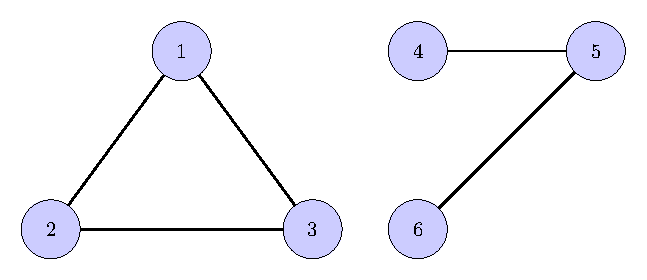
\includegraphics[scale=0.7]{tikz.pdf}
\caption{Graph, $\mathcal{G}$ with six nodes and two components.}
\end{center}
\end{figure}

\begin{enumerate}
\item (3 points) Create the adjacency matrix, ${\bf A}$, corresponding to $\mathcal{G}$. (Note that node $i$ should correspond to the $i$th row of {\bf A}. 
\item (2 points) We will go through some steps to write the code to compute the Graph Laplacian. The first matrix we need to define is the diagonal degree matrix, ${\bf D}$. Create the degree matrix (${\bf D}$) for $\mathcal{G}$. 
\item (2 points) Define the Laplacian matrix, ${\bf L}$ as ${\bf L}={\bf D}-{\bf A}$. 
\item (2 points) An eigenvector (${\bf v} \in \mathbb{R}^{6}$) and its corresponding eigenvalue ($\lambda$) of the graph Laplacian, ${\bf L}$, must satisfy ${\bf L}{\bf v} = \lambda {\bf v}$. As this graph has two components, we will be able to find two unique eigenvectors (${\bf v}_{1}$ and ${\bf v}_{2}$) that correspond to the zero eigenvalue, such that ${\bf L} \times {\bf v}_{1} = 0 \times {\bf v}_{1} $ and ${\bf L} \times {\bf v}_{2} = 0 \times {\bf v}_{2} $. Consider ${\bf v}_{1} = [1, 1, 1, 0, 0, 0]^{T}$. You will notice that there are 1s in the first three entries, corresponding to the nodes that are together in a component. Check that ${\bf v}_{1}$ does indeed correspond to eigenvalue 0 and satisfies ${\bf L} \times {\bf v}_{1} = 0 \times {\bf v}_{1} $. 

If you are using numpy, you can check by computing, 
\begin{center}
\begin{verbatim}
L @ np.matrix([[1],[1],[1],[0],[0],[0]])
\end{verbatim} 
\end{center}

Discuss your findings.
\item (3 points) Given this pattern you just observed with ${\bf v}_{1}$, find ${\bf v}_{2}$. Show that your ${\bf v}_{2}$ satisfies ${\bf L} \times {\bf v}_{2} = 0 \times {\bf v}_{2} $. 

You can fill in the following with your entries of ${\bf v}_{2}$. 
\begin{center}
\begin{verbatim}
L @ np.matrix([[ ],[ ],[ ],[ ],[ ],[ ]])
\end{verbatim} 
\end{center}

\item (2 points) As a further numerical experiment, find the eigenvalues of ${\bf L}$ (you can use  \url{https://numpy.org/doc/stable/reference/generated/numpy.linalg.eig.html#numpy.linalg.eig}). What do you notice about the smallest two eigenvalues? What about the third smallest eigenvalue? 

\end{enumerate}

\end{homeworkProblem}


%\end{equation}
\begin{homeworkProblem}
({\bf A Single-Cell Graph in the Wild}) (3 points) 
A graph, $\mathcal{G}_{cell}$ was constructed between 5000 cells contained in \path{cell_graph.edgelist}. Make sure for the subsequent problems you interpret this as an undirected graph and the adjacency matrix is symmetric. 
\begin{itemize}
\item (3 points) Use all of your hard work from Problem 2 to compute the graph Laplacian, ${\bf L}$ for $\mathcal{G}_{cell}$.  Make a histogram to visualize the distribution of eigenvalues of ${\bf L}$. What is the smallest eigenvalue of ${\bf L}$? What are the smallest and second smallest eigenvalues of ${\bf L}$ and how does the observation relate to the structure of the graph? 
 \end{itemize}
\end{homeworkProblem}

\begin{homeworkProblem} (14 Points Total)
\begin{figure}
\begin{center}
\includegraphics[scale=0.2]{cellGraph}
\caption{A visualization of the graph in homework problem 3.}
\end{center}
\end{figure}
{\bf Playing with Single Cell Data}\\
We will consider data from a CyTOF experiment obtained from \url{http://flowrepository.org/id/FR-FCM-ZZPH}. Here, we are considering the expression of 13 different protein markers across a set of cells. It has already been pre-processed for you. From the entire dataset, 5,000 cells were sampled for further analysis. You can use the following accompanying data as follows. 
\begin{itemize}
\item \path{Levine_matrix.csv} is the cell $\times$ marker matrix. Note that the last column is labels for the cells. Let's call this matrix, ${\bf X}$. \textcolor{blue}{\bf You should not use the last column (named label) for any kind of clustering.} Some cells are not labeled (hence are called NaN).
\item \path{population_names_Levine_13dim.txt} maps the cell labels from the last column of ${\bf X}$ (number labels) to biologically-interpretable cell-type names. 
\item \path{cell_graph.edgelist} is an edgelist for a between-cell graph. We will call this, {\bf G}. Note that the nodes in ${\bf G}$ correspond to the rows in ${\bf X}$. So, node $i$ maps to row $i$ of ${\bf X}$, etc.
\end{itemize}

1) {\bf Clustering on cell $\times$ marker data} (7 points): Use a clustering algorithm of your choice to generate a cell-to-cluster partition for the cells, using the matrix, ${\bf X}$. Use normalized mutual information (NMI) to compute overlap between the true and predicted cell labels. \textcolor{blue}{\bf Note that because not all cells are labeled, you can compute this only based on the labeled cells.} Feel free to use an available implementation, such as, \url{https://scikit-learn.org/stable/modules/generated/sklearn.metrics.normalized_mutual_info_score.html}. \\

2) {\bf Graph Partitioning} (7 points): Use a graph clustering algorithm to partition ${\bf G}$ into clusters. Similar to part 1 (1) compute NMI between the labels obtained in graph partitioning and the true cell labels. \\

3) (3 points) Comment on any observations you observe between the quality of the partitions obtained clustering on ${\bf X}$ in comparison to partitioning ${\bf G}$. Which approach do you think works better, using the original data, or the graph? \\

4) {\bf Rare Cell-types} (5 points) \path{Plasmacytoid_DC_cells}, or pDCs (label 21) are a popular rare cell type, meaning many clustering algorithms will not be able to reliably find them. Report the number of distinct clusters where you found pDCs in both the clustering of ${\bf X}$ and in the partitioning of ${\bf G}$.  \\

5) {\bf Cell Classification} (10 points) Select cells from ${\bf X}$ with the following labels, $\{11, 12, 17, 18\}$ and $\{1,2,3\}$. In general, cells with labels $\{11, 12, 17, 18\}$ are T-cells and cells with labels $\{1,2,3\}$ are monocytes. Convert this to a binary classification problem by labeling T-cells with 0 and monocytes with 1. Use your favorite classifier to predict the labels of these cells. Use an ROC curve to visualize the performance. Please be sure to use an appropriate training/testing or cross validation procedure.  If the performance was not good, explain what could have gone wrong. If your performance is very good, can you identify features from ${\bf X}$ that were helpful in predicting labels?

\end{homeworkProblem}

\begin{homeworkProblem}
(30 points total) {\bf node2vec} \\

We will use the implementation of node2vec available in github, \url{https://github.com/eliorc/node2vec}.  \\

1) ({\bf Clustering on Node2Vec Features} (10 points)) First, use default parameters and follow the instructions in the README on the graph in \path{cell_graph.edgelist}. This will create a 128-dimensional vector for each node. Cluster the nodes based on these vectors and compare to the ground truth labels in the last column of \path{Levine_matrix.csv} using NMI. Compare your results to Problem 4, question 3. Does an embedding of the graph offer any apparent advantages in classifying cells? \\

2) ({\bf Parameters, part 1} (5 points)) Try a few different values for the number of dimensions \path{--dimensions}, such that some of them are less than 128, and some of them are more than 128. Cluster cells again with the embeddings obtained in different dimensions. Again, you can compute the NMI between the cluster assignments and the ground truth labels. Comment on some observations, and show a plot of NMI plotted against the number of dimensions used. \\

3) ({\bf Parameters, part 2} (5 points)) Recall that the parameters $p$ and $q$ control the `breadth' vs `depth of the walk'. Choose one of these parameters to vary, and repeat the previous question using the default 128 dimensions, but varying values for either $p$ or $q$. Comment on some observations, and show a plot of NMI against $p$ or $q$ (whichever one you chose). \\

4) ({\bf Cell Classification, Part II} (10 points)) Repeat Problem 4, question (5). However, instead of using only ${\bf X}$ as the feature matrix, we are going to combine the marker expressions with node2vec features. Let ${\bf N}$ be your matrix generated through node2Vec. Create a new matrix called ${\bf X}=[{\bf X} | {\bf N}]$. That is, you will simply concatenate ${\bf X}$ and ${\bf N}$. Formulate the same classification problem from Problem 4, question (5) to classify T-cells from monocytes. Again, report your ROC curve. Please use an appropriate training/testing or cross-validation procedure. Comment on the performance, especially in comparison to the results obtained in Problem 4, question (5). 

\end{homeworkProblem}

\end{document}